\begin{frame}{Background: Max Entropy RL}
\textbf{Conventional RL Objective --- Expected Reward}
\[
\sum_{t} \mathbb{E}_{(\mathbf{s}_t, \mathbf{a}_t) \sim \rho_\pi}\!\left[ r(\mathbf{s}_t, \mathbf{a}_t) \right]
\]

\textbf{Maximum Entropy RL Objective --- Expected Reward + Entropy of Policy}
\[
\sum_{t} \mathbb{E}_{(\mathbf{s}_t, \mathbf{a}_t) \sim \rho_\pi}\!\left[ r(\mathbf{s}_t, \mathbf{a}_t) + \alpha\, \textcolor{red}{\mathcal{H}(\pi(\,\cdot \mid \mathbf{s}_t))} \right]
\]

\textbf{Entropy of a RV $x$}
\[
H(P) = \mathbb{E}_{x \sim P}\!\left[ -\log P(x) \right]
\]
\end{frame}
\begin{frame}{Max Entropy RL}
\begin{itemize}
    \item MaxEnt RL agent can capture different modes of optimality to improve robustness against environmental changes
\end{itemize}
\begin{columns}[c]
\begin{column}{0.5\textwidth}
\centering
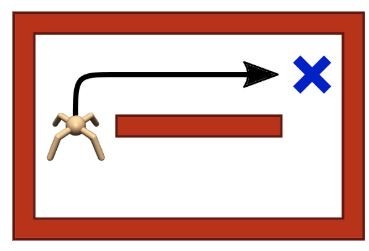
\includegraphics[width=0.9\linewidth,height=0.32\textheight,keepaspectratio]{images/soft-actor-critic/figures/maxent-maze-left.jpg}\\
\vspace{0.2em}
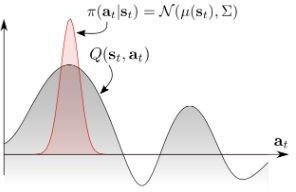
\includegraphics[width=0.9\linewidth,height=0.32\textheight,keepaspectratio]{images/soft-actor-critic/figures/maxent-gauss-left.jpg}
\end{column}
\begin{column}{0.5\textwidth}
\centering
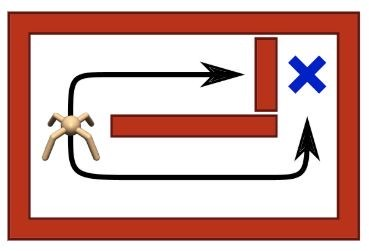
\includegraphics[width=0.9\linewidth,height=0.32\textheight,keepaspectratio]{images/soft-actor-critic/figures/maxent-maze-right.jpg}\\
\vspace{0.2em}
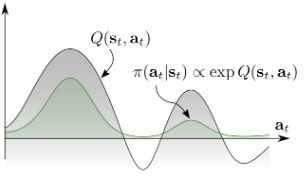
\includegraphics[width=0.9\linewidth,height=0.32\textheight,keepaspectratio]{images/soft-actor-critic/figures/maxent-gauss-right.jpg}
\end{column}
\end{columns}
\begin{flushright}
    \tiny\url{https://bair.berkeley.edu/blog/2017/10/06/soft-q-learning/}
\end{flushright}
\end{frame}
\begin{frame}{Max Entropy RL}
\begin{columns}[c]
\begin{column}{0.4\textwidth}
\centering
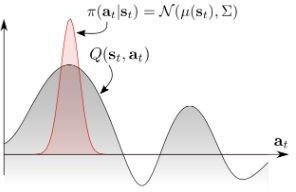
\includegraphics[width=0.95\linewidth,height=0.32\textheight,keepaspectratio]{images/soft-actor-critic/figures/maxent-derivation-plot-uni.jpg}\\
\vspace{0.4em}
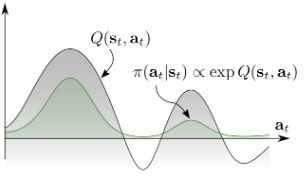
\includegraphics[width=0.95\linewidth,height=0.32\textheight,keepaspectratio]{images/soft-actor-critic/figures/maxent-derivation-plot-multi.jpg}
\end{column}
\begin{column}{0.58\textwidth}
\small
\begin{align*}
&\min_{\pi} D_{\mathrm{KL}}\big(\pi(\,\cdot \mid s_0) \,\|\, \exp(Q(s_0, \cdot))\big) \\
&= \min_{\pi} \mathbb{E}_\pi\!\left[ \log \frac{\pi(a_0 \mid s_0)}{\exp(Q(s_0, a_0))} \right] \\
&= \max_{\pi} \mathbb{E}_\pi\!\left[ Q(s_0, a_0) - \log \pi(a_0 \mid s_0) \right] \\
&= \max_{\pi} \mathbb{E}_\pi\!\left[ \sum_t r(s_t, a_t) + \mathcal{H}(\pi(\,\cdot \mid s_0)) \mid s_0 \right] \\
&= J_{\mathrm{MaxEnt}}(\pi(\,\cdot \mid s_0))
\end{align*}
\end{column}
\end{columns}
\end{frame}
